\documentclass[12pt,letterpaper]{article}
\usepackage{cite}
\usepackage{amsmath}
\usepackage{amsfonts}
\usepackage{array}
\usepackage{dsfont}
\usepackage{amssymb}
\usepackage{amsthm}
\usepackage{bbold}
\usepackage{fullpage}
\usepackage{mathtools}
\usepackage{enumitem}
\usepackage{mathrsfs}
\usepackage[margin=0.9 in]{geometry}
\usepackage{hyperref}
\usepackage{graphicx}
\usepackage{gensymb}
\usepackage{xcolor,colortbl}
\usepackage[format=plain,
labelfont={bf,it},
textfont={it}]{caption}
\usepackage{float}


\newcommand*{\SignatureAndDate}[1]{%
	\par\noindent\makebox[2.5in]{\hrulefill} \hfill\makebox[2.0in]{\hrulefill}%
	\par\noindent\makebox[2.5in][l]{#1}      \hfill\makebox[2.0in][l]{Date}%
}%
\newcolumntype{L}{>{\centering\arraybackslash}m{2cm}}
\newcolumntype{P}{>{\centering\arraybackslash}m{3cm}}
\newcolumntype{Q}{>{\centering\arraybackslash}m{4cm}}
\setlength{\parindent}{0em}

\allowdisplaybreaks

\newcommand{\R}{\mathds{R}}
\newcommand{\Z}{\mathds{Z}}
\newcommand{\Rplus}{\mathds{R}_{> 0}}
\newcommand{\Zplus}{\mathds{Z}_{\geq 0}}
\newcommand{\F}{\mathds{F}}
\newcommand{\N}{\mathds{N}}
\newcommand{\T}{\mathds{T}}
\newcommand{\s}{\mathds{S}}
\newcommand{\C}{\mathds{C}}
\newcommand{\CDFT}{\mathscr{F}_{CD}} %Fourier transform
\newcommand{\ip}[2]{\langle #1, #2\rangle}


\setlength{\parskip}{0.5em}


\makeatletter
\newsavebox\myboxA
\newsavebox\myboxB
\newlength\mylenA

\begin{document}
	
\section{Technical Background}
A number of mathematical tools were utilized to develop the framework necessary for the mathematical modelling and control of the RipStik.

\subsection{Euler Angles}

Euler angles were introduced to describe the orientation of a body in an inertial reference frame.
These orientations were represented by rotations of three angles; yaw ($\theta$), pitch ($\psi$), and roll ($\alpha$).
With the Euler angles defined, rotation matrices can then be created for the bodies of a system.

A rotation matrix can be defined in the following way \cite{Lewis}:

\begin{equation}
\label{eq:RotM}
 R =
\begin{bmatrix} 
\cos\alpha\cos\psi & \cos\alpha\sin\psi\sin\theta - \cos\theta\sin\alpha &\cos\alpha\cos\theta\sin\psi+\sin\alpha\sin\theta\\
\cos\psi\sin\alpha & \cos\alpha\cos\theta+\sin\alpha\sin\psi\sin\theta & \cos\theta\sin\alpha\sin\psi - \cos\alpha\sin\theta\\
-\sin\psi & \cos\psi\sin\theta & \cos\psi\cos\theta 
\end{bmatrix}
\end{equation}

The rotation matrix R can be used to describe a rotation from a body-fixed frame to the inertial frame \cite{VTOL}.

\subsection{Lagrangian Mechanics}

Lagrangian mechanics can be used in place of Newtonian mechanics when trying to accurately model highly complex systems.
In these elaborate systems, constraint forces can be implemented to eliminate degrees of freedom and reduce the complexity of the system \cite{LagrangeEquations}. Additionally, Lagrangian equations are invariant to changes of coordinate systems \cite{LagrangePowerpoint}.
\par
The Lagrangian function is represented by L, and is defined as the difference between kinetic and potential energies in a system modeled using positions and velocities \cite{NonholonomicPowerpoint}.
In the equation, T represents the kinetic energy and V represents the potential energy.
The mathematica formulation for the Lagrangian follows:

\begin{equation}
\label{eq:Lagrange}
L = T - V
\end{equation}

\subsection{Euler-Lagrange Equations}
The Lagrangian can then be applied to the Euler-Lagrange equations to solve for the equations of motion in the system. 
A mathematical representation of the Euler-Lagrange equations follows:

\begin{equation}
\label{eq:EL}
\frac{\text{d}}{\text{dt}} \bigg(\frac{\partial \text{L}}{\partial \dot{\text{q}}_{i}}\bigg) - \frac{\partial \text{L}}{\partial \text{q}_{i}} = 0
\end{equation}
The Euler-Lagrange equations are equivalent to Newton's second law \cite{NonholonomicPowerpoint}, and are implicit second-order differential equations applied to a given coordinate system \cite{Lewis}.
\par
The unconstrained equations of motion encompass each degree of freedom in the system, and are of the following form:

\begin{equation}
\label{eq:UEOM}
G_{jk} \ddot{q}^k + \Gamma_{jkl} \dot{q}^k\dot{q}^l  = F_{j}
\end{equation}

In equation \ref{eq:UEOM}, $G_{jk}$ represents the acceleration coefficients of the system, $\Gamma_{jk}$ represents the velocity coefficients of the system, and $F_j$ represents the potential forces of the system.

\subsection{Nonholonomic Constraints}
Nonholonomic constraints can be implemented to restrict velocities in a system \cite{LagrangeEquations}.
Lagrange multipliers can be added to the unconstrained equations of motion to represent unknown constraint forces \cite{ClassicalMechanics}.
\par
The forces can then be determined from the following system of equations:

\begin{equation}
\label{eq:CFE}
G_{jk} \ddot{q}^k + \Gamma_{jkl} \dot{q}^k\dot{q}^l  = \lambda_{a}\omega_{j}^{a} + F_{j}
\end{equation}

\begin{equation}
\label{eq:CV}
\omega_{j}^{a} \dot{q}^{j} = 0
\end{equation}

Equation \ref{eq:CFE} is identical to the unconstrained equations of motion with the added $\lambda_{a}$ term, representing the constraint forces.
Equation \ref{eq:CV} represents the constrained velocity terms. 
\par
When solving for the constraint forces, the system takes on the form of a Differential Algebraic Equation (DAE).

\subsection{Numeric Integration}
Numeric Integration allows for the approximate computation of an integral using numerical methods \cite{WolframNumeric}.
When applying numeric integration to a differential system, stiffness is often a by-product.
The concept of stiffness is not well understood, but can generally be attributed to quick changing dynamics in a system \cite{StiffSystem}.
\par
To help develop some intuition on how stiff systems work, an example can be seen in figure \ref{fig:stiffsystem}.

\begin{figure}[!htb]
	\centering
	\minipage{0.7\textwidth}
	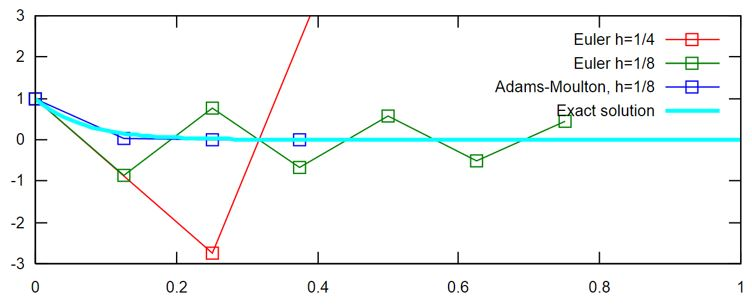
\includegraphics[width=\linewidth]{stiffsystem}
	\caption{Using numeric integration methods to approximate the exact solution to a differential equation}\label{fig:stiffsystem}
	\endminipage
\end{figure}
figure \ref{fig:stiffsystem} shows the exact output from a simple differential equation in light blue. 
When numeric integration is attempted using Euler's method and a step size of 1/4, the approximation oscillates and completely overshoots the exact method as seen in red. 
When a step size of 1/8 is selected, there are still oscillations, but they are in a reasonable range around the exact solution as seen in green. 
When adams-Moulton method is used with a step size of 1/8, the oscillations are essesntially negligible and the approximation is almost equal to the exact solution.


\par
When a system has quickly changing dynamics, numeric integration will require increasingly small step sizes to approximate a solution without instability \cite{StiffSystem}. 
This adds computational complexity that ofteen exceeds modern technological capabilities. 
To try and reduce this computational complexity, four different numerical methods were selected to evaluate stiff DAE systems.

The QR Decomposition method decomposes the Jacobian of the derivative, breaking down the core system into two smaller systems at each iteration point \cite{Methods}.
This is represented by the following equation:

\begin{equation}
\label{eq:QR}
A = QR
\end{equation}

In equation \ref{eq:QR}, A is any real square matrix, Q is an orthogonal matrix, and R is an upper triangular matrix \cite{Methods}.

The Collocation method linearizes the implicit DAE to m points in time, generating a system of linear equations which can be solved iteratively using Newton's Method \cite{Methods}.
The Implicit Differential-Algebraic Method uses Backward Differential Formulas (BDF) to implicity solve the DAE for derivatives to use an ODE solver \cite{Methods}. 
The BDF approximates the derivative of the function using information from previous time steps \cite{Methods}.
The BLT Method puts the system into block lower triangular form and solves subsets of the system iteratively \cite{Methods}.



\newpage
\bibliography{Bibliography}{}
\bibliographystyle{unsrt}

\end{document} 